\scanpage{160}
% position: top two sequences
\diagram{\begin{tikzcd}
0\arrow[r,dash]&\unsure{\deleted{E_1}\inserted{L_1}}\arrow[r,dash]&E_1\arrow[r,dash]&\unsure{L'_1}\arrow[r,dash]&0\\
0\arrow[r,dash]&L_2^{\unsure{4|+}}\arrow[r,dash]&E_2\arrow[r,dash]&L'_2\arrow[r,dash]&0
\end{tikzcd}}
% position: upper right note
\margin{\(L_1,L'_1\) \unsure{qcq} \unsure{ici.}\par
\unsure{non.} Mais \unsure{suppos.} \(L'_1,L'_2\)
loc. libres de rang fini}
% position: left mark by middle sequence
\margin{\unsure{\(\longrightarrow\)|-}}
% position: middle sequence
\diagram{\begin{tikzcd}
0\arrow[r,dash]&L_1^{\unsure{4|+}}\otimes L_2\arrow[r,dash]&E_1\wedge E_2\arrow[r,dash]&L'_1\otimes L'_2\arrow[r,dash]&0
\end{tikzcd}}
% position: dual sequence
\diagram{\begin{tikzcd}
0&L_1^\vee\otimes L_2^\vee\arrow[l]&E_1^\vee\wedge E_2^\vee\arrow[l]&L_1'{}^\vee\otimes L_2'{}^\vee\arrow[l]&0\arrow[l]
\end{tikzcd}}
\figure{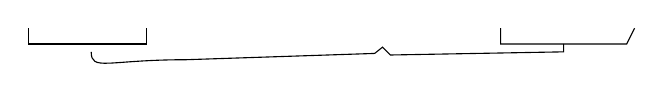
\begin{tikzpicture}
\draw (0,.2)--(0,0)--(1.5,0)--(1.5,.2);
\draw (6,.2)--(6,0)--(7.6,0)--(7.7,.2);
\draw (.8,-.1)..controls (.8,-.35) and (1,-.2)..(2,-.2)--(4.4,-.12)--(4.5,-.04)--(4.6,-.14)--(6.8,-.1)--(6.8,0);
\end{tikzpicture}}
% position: middle assertion
Je dis que
\[
E_1^\vee\wedge E_2^\vee\simeq(E_1\wedge E_2)^\vee
\]
% position: Hom expression
\[
\operatorname{Hom}(L'_1,\unsure{k|\mathcal O})\otimes\operatorname{Hom}(L'_2,\unsure{k|\mathcal O})
\simeq\operatorname{Hom}(L'_1\otimes L'_2,\unsure{k|\mathcal O})
\]
% position: lower initial pairing
\[
\unsure{f_1}\otimes f_2+\bar f_1\otimes\bar f_2,\quad x_1\otimes x_2
\]
% position: lower left diagram
\diagram{\begin{tikzcd}[row sep=small,column sep=large]
\unsure{A|\mathcal A}_1\otimes\unsure{A|\mathcal A}_2\arrow[dd,Rightarrow]\arrow[dr] &\\
&\unsure{A|\mathcal A}_1\otimes\unsure{A|\mathcal A}_2\\
L_1\otimes L_2\arrow[ur,"\begin{gathered}\pi_1\otimes\mathrm{id}\\\mathrm{id}\otimes\pi_2\end{gathered}"']&
\end{tikzcd}}
% position: lower middle trace products
\[
\begin{aligned}
&(\operatorname{Tr}_1(f_1)-f_1)\otimes(\operatorname{Tr}_2(\unsure{f_2})-\unsure{f|f_2})\\
&(\pi'_1(f_1)-f_1)(\pi_2(\unsure{f_2})-\unsure{f|f_2})
\end{aligned}
\]
% position: isolated f signs
\[
\unsure{f_4|\deleted{f_4}}\qquad\unsure{f_2|\deleted{f_2}}\qquad f_1
\]
% position: lower left pi fragments
\margin{\(\pi_1(x_1)-\)}
% position: lower sigma expressions
\[
\deleted{\sigma=\unsure{\pi}}\qquad\sigma(x)=\operatorname{Tr}(x).1-x
\]
\[
\sigma\equiv T\otimes\unsure{\ell|e}-\mathrm{id}
\]
% position: right sloping marginal formulas
\margin{\(\begin{gathered}
2x-\psi(x)T\\
\uline{x-\psi(x)T}\\
=-\sigma(x)
\end{gathered}\)}
% position: lower left second pi fragment
\margin{\(\pi_1(x_1)\)}
% position: lower right isolated trace expression
\margin{\(u_1\otimes\uline{\operatorname{Tr}(x_2)}=\unsure{i|1}\)}
% position: lower tensor maps
\[
\begin{aligned}
\unsure{u_1|x_1}\otimes x_2&\longmapsto\deleted{\unsure{\pi_1}(\unsure{x_1|u_1})\otimes x}\quad u_1\otimes\pi_2(x_2)\\
x_1\otimes u_2&\unsure{\vdash|\longmapsto}\pi_1(x_1)\otimes u_2
\end{aligned}
\]
% position: bottom boxed tensor expression
\[
\boxed{x_1\otimes x_2+\pi'_1(x_1)\otimes\pi'_2(x_2)}
\]
% position: bottom right marginal computation
\margin{\(\unsure{(\chi-1)x|(\chi-1)^x}\)
\figure{\begin{tikzpicture}\draw[->] (.8,.5)..controls (.9,.05) and (.15,.3)..(0,0);\end{tikzpicture}}
\(\pi_2(x)=\unsure{x|\bar x}+\pi'_2(x)\)
\(\left\{\begin{array}{l}
\text{Si }x\in L_2,\ \text{\unsure{on}.}\\
\pi'_2(\unsure{x})=\unsure{x}
\end{array}\right.\)}
% position: foot pencil
\margin{159}
